\documentclass[border=6pt]{standalone}
\usepackage[T1]{fontenc}
\usepackage{courier}
\usepackage[scaled=0.95]{helvet}
\renewcommand{\familydefault}{\sfdefault}
\usepackage{sfmath}
\usepackage[version=4]{mhchem}
\usepackage{tikz}
\usepackage{pgfplots}
\pgfplotsset{compat=newest}
\usetikzlibrary{arrows.meta,positioning,calc,fit,backgrounds,shapes.geometric,decorations.pathreplacing,patterns}
\definecolor{ink}{HTML}{17233A}
\definecolor{inksoft}{HTML}{44506A}
\definecolor{teal}{HTML}{0E6B6B}
\definecolor{tealsoft}{HTML}{E5F0EF}
\definecolor{amber}{HTML}{B26B12}
\definecolor{ambersoft}{HTML}{FBF0DF}
\definecolor{blue}{HTML}{2F6690}
\definecolor{bluesoft}{HTML}{E3ECF4}
\definecolor{plum}{HTML}{7A4D8C}
\definecolor{plumsoft}{HTML}{EFE7F3}
\definecolor{greyc}{HTML}{8A94A3}
\definecolor{linec}{HTML}{D3DCE1}
\definecolor{oxy}{HTML}{C0392B}
\definecolor{carb}{HTML}{3B4252}
\definecolor{hyd}{HTML}{E6E9EE}
\definecolor{nit}{HTML}{2F6690}
\tikzset{
  every picture/.style={line cap=round,line join=round},
  lab/.style={font=\small, text=inksoft},
  >={Stealth[length=7pt]},
}
\pgfplotsset{
  every axis/.append style={axis line style={inksoft}, tick style={inksoft}, tick label style={font=\footnotesize, text=inksoft}, label style={font=\small, text=ink}},
}
% fragment tile: \frag{node name}{position}{colour}{content}
\newcommand{\frag}[4]{\node[draw=#3, fill=#3!12, line width=1.4pt, rounded corners=6pt, minimum width=1.25cm, minimum height=1.05cm, text=#3, font=\bfseries] (#1) at (#2) {#4};}
\newcommand{\ring}{\tikz[baseline=-0.6ex]{\draw[line width=1.1pt] (0:0.3)--(60:0.3)--(120:0.3)--(180:0.3)--(240:0.3)--(300:0.3)--cycle; \draw[line width=0.8pt] (0,0) circle (0.16);}}
\newcommand{\bond}[2]{\draw[ink, line width=2.2pt] (#1) -- (#2);}

\begin{document}
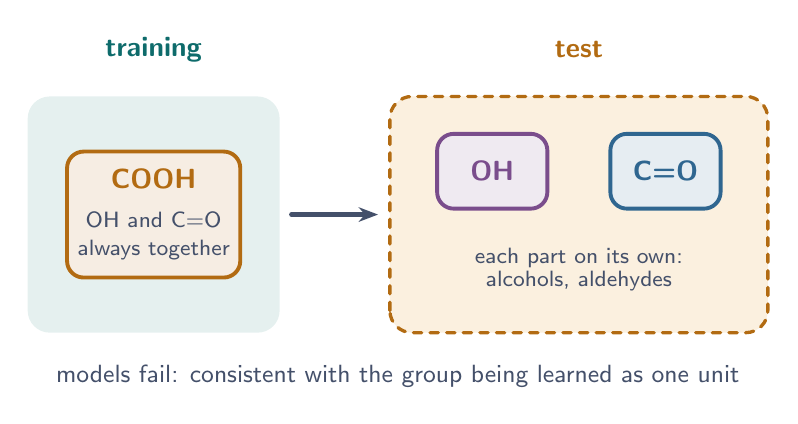
\begin{tikzpicture}
\node[font=\bfseries, text=teal] at (1.6,3.0) {training};
\node[font=\bfseries, text=amber] at (7.0,3.0) {test};
\fill[tealsoft, rounded corners=8pt] (0,-0.6) rectangle (3.2,2.4);
\draw[amber, dashed, line width=1.2pt, fill=ambersoft, rounded corners=8pt] (4.6,-0.6) rectangle (9.4,2.4);
\node[draw=amber, fill=amber!12, line width=1.4pt, rounded corners=6pt, minimum height=1.6cm, minimum width=2.2cm, align=center, font=\bfseries, text=amber] at (1.6,0.9) {COOH\\[2pt]{\footnotesize\mdseries\textcolor{inksoft}{OH and C=O}}\\[-2pt]{\footnotesize\mdseries\textcolor{inksoft}{always together}}};
\draw[->, inksoft, line width=1.7pt] (3.35,0.9) -- (4.45,0.9);
\node[draw=plum, fill=plum!12, line width=1.4pt, rounded corners=6pt, minimum height=0.95cm, minimum width=1.4cm, font=\bfseries, text=plum] at (5.90,1.45) {OH};
\node[draw=blue, fill=blue!12, line width=1.4pt, rounded corners=6pt, minimum height=0.95cm, minimum width=1.4cm, font=\bfseries, text=blue] at (8.10,1.45) {C=O};
\node[font=\footnotesize, text=inksoft, align=center] at (7.0,0.2) {each part on its own:\\[-1pt]alcohols, aldehydes};
\node[font=\small, text=inksoft] at (4.7,-1.15) {models fail: consistent with the group being learned as one unit};
\end{tikzpicture}
\end{document}
